
\documentclass[a4paper,12pt]{article}

\usepackage{graphicx}
\usepackage{amssymb}
\usepackage{amsmath}
\usepackage{amsfonts}

\usepackage{placeins}

\usepackage[hidelinks]{hyperref}
\usepackage{url}


\usepackage[english]{babel}
\usepackage{booktabs}
\usepackage{stfloats}
\usepackage[T1]{fontenc}

\usepackage{float}
\restylefloat{table}

\usepackage{longtable}

\usepackage{xcolor,colortbl}

\usepackage{mathpazo} % Palatino
\usepackage{avant}           % Avant Garde

\usepackage[margin=2cm]{geometry}
%\usepackage[landscape]{geometry}

\renewcommand{\vec}[1]{\mathbf{#1}}

\setlength\parindent{0pt}

\newcommand{\HRule}[1]{\hfill \rule{0.2\linewidth}{#1}}

\definecolor{Gray}{gray}{0.90}




\begin{document}


\thispagestyle{empty} % Remove page numbering on this page

%----------------------------------------------------------------------------------------
%	TITLE SECTION
%----------------------------------------------------------------------------------------

\colorbox{Gray}{
	\parbox[t]{1.0\linewidth}{
		\centering \fontsize{50pt}{80pt}\selectfont % The first argument for fontsize is the font size of the text and the second is the line spacing - you may need to play with these for your particular title
		\vspace*{0.7cm} % Space between the start of the title and the top of the grey box

		\hfill PyECLOUD \\
		\hfill Reference \\
		\hfill Manual\par

		\vspace*{0.7cm} % Space between the end of the title and the bottom of the grey box
	}
}

%----------------------------------------------------------------------------------------

\vfill % Space between the title box and author information

%----------------------------------------------------------------------------------------
%	AUTHOR NAME AND INFORMATION SECTION
%----------------------------------------------------------------------------------------

{\centering \large
\hfill Giovanni Iadarola, \\
\hfill Eleonora Belli, Philipp, Dijkstal,\\
\hfill Lotta Mether, Annalisa Romano,\\
\hfill Giovanni Rumolo Eric Wulff\\
\hfill CERN - Geneva, Switzerland

\HRule{1pt}} % Horizontal line, thickness changed here

%----------------------------------------------------------------------------------------

\clearpage % Whitespace to the end of the page

\newpage

\section*{PyECLOUD reference manual}

This document describes the main input and output parameters for the PyECLOUD code for the simulation of the electron cloud buildup in particle accelerators.

\section{Input files}
\subsection{Simulation parameters}

This input file has to be named \textbf{simulation\_parameters.input}.

\renewcommand*{\arraystretch}{1.4}
\begin{longtable}
{p{0.42\textwidth}p{0.53\textwidth}}
\hline\endfirsthead\hline\endhead
\rowcolor{Gray}\multicolumn{2}{p{.97\textwidth}}{
\textbf{Other input filenames.} The following variables specify the names of the other three input files which define the physical model of the simulation.}\\
\hline
\textbf{machine\_param\_file} & Name of the machine parameter file.\\
\hline
\textbf{secondary\_emission\_parameters\_file} & Name of the secondary emission configuration file. \\
\hline
\textbf{beam\_parameters\_file} & Name of the beam parameter file (in case of a multiple beam simulation this is the master beam).\\
\hline
\end{longtable}


\begin{longtable}
{p{0.42\textwidth}p{0.53\textwidth}}
\hline\endfirsthead\hline\endhead
\rowcolor{Gray}\multicolumn{2}{p{.97\textwidth}}{
\textbf{Secondary beams} The code can simulate the EC buildup in the presence of more than one circulating beam. For this purpose a list of secondary beam files (one for each beam) has to be provided.
In the presence of secondary beams, the master beam determines the length of the simulation, the energy used for the calculation of the bending field, and the bunch spacing used for regeneration and saving purposes.
}\\
\hline
\textbf{secondary\_beam\_file\_list} & (optional -- default = []) \newline List of names of secondary beam parameter files.\\
\hline
\end{longtable}

\begin{longtable}
{p{0.42\textwidth}p{0.53\textwidth}}
\hline\endfirsthead\hline\endhead
\rowcolor{Gray}\multicolumn{2}{p{.97\textwidth}}{
\textbf{Log and progress files}
}\\
\hline
\textbf{logfile\_path} &	Path of a text file that reports some synthetic information on the ongoing simulation (Passage number, number of MPs and number of electrons in the chamber).\\
\hline
\textbf{progress\_path} &	Path of a text file that reports the simulation progress in percent.\\
\hline
\end{longtable}



\begin{longtable}{p{0.42\textwidth}p{0.53\textwidth}}
\hline\endfirsthead\hline\endhead
\rowcolor{Gray}\multicolumn{2}{p{.97\textwidth}}{
\textbf{Time sampling} The simulated time interval is defined by the length of the beam profile (number of bunch passages) specified in the beam description.
}\\
\hline
\textbf{Dt} & [s] Simulation time step. This input is not considered if beam profile is imported from file.\\
\hline
\textbf{t\_end} & [s] Extra time interval after the specified beam profile.

Only coasting beam present in this interval. The value of this variable can also be negative in order to stop the simulation before the end of the specified profile. \\
\hline
\end{longtable}


\begin{longtable}{p{0.42\textwidth}p{0.53\textwidth}}
\hline\endfirsthead\hline\endhead
\rowcolor{Gray}\multicolumn{2}{p{.97\textwidth}}{
\textbf{Negligible beam linear density} }\\
\hline
\textbf{lam\_th} & [beam part/m] When the linear density of the beam is below this value,
primary electrons are not generated and beam forces on the electrons are neglected.\\
\hline
\end{longtable}



\begin{longtable}{p{0.42\textwidth}p{0.53\textwidth}}
\hline\endfirsthead\hline\endhead\rowcolor{Gray}
\multicolumn{2}{p{.97\textwidth}}{
\textbf{MP management settings}
}\\ \hline
\textbf{N\_mp\_max}&	Size of the arrays allocated to store the MP sizes, positions and velocities. MP regeneration settings must be set such that this number of MPs is never exceeded.\\ \hline
\textbf{N\_mp\_regen}& 	MP regeneration threshold. When the total number of MPs exceeds N\_mp\_regen a regeneration of the set of MPs is applied and a new Nref is chosen in order to get a target number of MPs. The check is performed at each t=n*b\_spac with n an integer.\\ \hline
\textbf{N\_mp\_regen\_low}&	Lower MP regeneration threshold. When the total number of MPs becomes smaller than N\_mp\_regen\_low a regeneration of the set of MPs is applied and a new Nref is chosen in order to get a target number of MPs. The check is performed at each t=n*b\_spac with n an integer.\\ \hline
\textbf{t\_ON\_regen\_low}&	For t< t\_ON\_regen\_low the lower MP regeneration check is not performed.\\ \hline
\textbf{N\_mp\_after\_regen}&	Target number of MPs obtained after regeneration.\\ \hline
\textbf{fact\_split}&	MP split factor; when secondary emission occurs, if the size of the emitted charge is smaller than fact\_split*Nref, the impacting MP is simply rescaled according to the SEY. Otherwise new MPs are generated in order to keep the MP size as close as possible to Nref.\\ \hline
\textbf{fact\_clean}&	MP clean factor. MPs smaller than fact\_split*Nref are deleted from the MP set. This test is performed at each t=n*b\_spac with n an integer.\\ \hline
\textbf{nel\_mp\_ref\_0}&	[e-/m] Initial MP size.\\ \hline
\textbf{Nx\_regen, Ny\_regen, Nvx\_regen, Nvy\_regen, Nvz\_regen}&	Number of mesh points in each dimension for the generation of the uniform grid for the 5-D phase space used for the MP regeneration.\\ \hline
\textbf{regen\_hist\_cut}&	Defines a threshold value for the phase space density, below which no electrons are generated.\\ \hline
\textbf{N\_mp\_soft\_regen}&	(optional: by default soft regen is not applied, the presence of these inputs enables it)

Soft regeneration threshold. The check is performed at each t=n*b\_spac with n an integer. N\_mp\_soft\_regen should be smaller than N\_mp\_regen.\\ \hline
\textbf{N\_mp\_after\_soft\_regen}&	(optional: by default soft regen is not applied, the presence of these inputs enables it)

Target number of MPs obtained after a soft regeneration.\\
\hline
\end{longtable}


\begin{longtable}{p{0.42\textwidth}p{0.53\textwidth}}
\hline\endfirsthead\hline\endhead\rowcolor{Gray}
\multicolumn{2}{p{.97\textwidth}}{
\textbf{Space charge parameters}
}\\ \hline
\textbf{Dt\_sc}&	[s] Time step for the update of the electron space charge field map.\\ \hline
\textbf{Dh\_sc }&		[m] Grid size for the space charge PIC solver.\\ \hline
\textbf{t\_sc\_ON}& [s] Electron space charge forces are neglected for t<t\_sc\_ON -- normally t\_sc\_ON=0. \\ \hline
    \textbf{sparse\_solver} & [optional] choices are 'klu', 'scipy\_slu' [default] \\\hline
    \textbf{PyPICmode} & [optional] Options are 'FiniteDifferences\_ShortleyWeller' [default], 'ShortleyWeller\_WithTelescopicGrids', 'FiniteDifferences\_Staircase'
    \\ \hline
\end{longtable}


\begin{longtable}{p{0.42\textwidth}p{0.53\textwidth}}
	\hline\endfirsthead\hline\endhead
	\rowcolor{Gray}\multicolumn{2}{p{.97\textwidth}}{
		\textbf{Multigrid parameters}

		 To be used with PyPICmode = 'ShortleyWeller\_WithTelescopicGrids'
	}\\
	\hline
	\textbf{f\_telescope}&	Magnification factor between grids (it must be always $0<f<1$).\\ \hline
	\textbf{target\_grid}&		Target grid parameters. It is a dictionary containing: 'x\_min\_target', 'x\_max\_target', 'y\_min\_target', 'y\_max\_target' and 'Dh\_target'.
\\ \hline
	\textbf{N\_nodes\_discard}& Number of nodes at the edge of the internal grids which are discarded in the field interpolation (going to coarser grid). \\ \hline
	\textbf{N\_min\_Dh\_main}& Minimum size of the first internal grid in the $\Delta h$ of the main grid. \\
	\hline
\end{longtable}


\begin{longtable}{p{0.42\textwidth}p{0.53\textwidth}}
\hline\endfirsthead\hline\endhead\rowcolor{Gray}
\multicolumn{2}{p{.97\textwidth}}{
\textbf{Saving settings}
}\\ \hline
    \textbf{filen\_main\_outp} & Main output filename or path. (optional - default 'Pyecltest.mat') \\ \hline
    \textbf{dec\_fact\_out} & Output is saved only for every nth time step. \\ \hline
\textbf{Dx\_hist}& 	[m] Defines the binning for the saving of the horizontal histograms.\\ \hline
\textbf{r\_center}&	[m] Radius of a circle around the (0, 0) point (center of the chamber) for the calculation of the local central density.\\ \hline
\textbf{Dt\_En\_hist}&	[s] Time step used to store the energy spectrum  of the electrons impacting on the chamber.\\ \hline
\textbf{Nbin\_En\_hist}&	Number of bins used for the energy histogram.\\ \hline
\textbf{En\_hist\_max}& 	[eV] Maximum energy in energy spectrum. Larger energies are attributed to the last bin of the histogram.	\\ \hline
\textbf{flag\_lifetime\_hist}&   If set to True enables lifetime histogram (optional -- default=False).\\ \hline
\multicolumn{2}{p{.97\textwidth}}{If \textbf{flag\_lifetime\_hist} is set to True, the variables \textbf{Dt\_lifetime\_hist}, \textbf{Nbin\_lifetime\_hist} and \textbf{lifetime\_hist\_max} need to be set.}\\ \hline
\textbf{Dt\_lifetime\_hist}&	[s] Time step used to store the histogram of the electrons lifetime.\\ \hline
\textbf{Nbin\_lifetime\_hist}&	Number of bins used for the histogram of the electrons lifetime.\\ \hline
\textbf{lifetime\_hist\_max}& 	[s] Maximum lifetime in the histogram of the electrons lifetime. Larger lifetimes are attributed to the last bin of the histogram.	\\ \hline
\textbf{flag\_cos\_angle\_hist} & Save the cosine of the incident angle of impacting electrons. (optional -- default True) \\ \hline
\textbf{cos\_angle\_width} & Width of the histogram bins. (optional -- default 0.05) \\ \hline
\textbf{flag\_movie}&	(optional -- default=0)

(1 $\Rightarrow$ On, 0 $\Rightarrow$ Off) Saves files with the electron density distribution at each space charge evaluation.\\ \hline
\textbf{flag\_sc\_movie}&	(optional-- default=0)

(1 $\Rightarrow$ On, 0 $\Rightarrow$ Off) Saves files with the electron space charge electric field distribution at each space charge evaluation.\\ \hline
\textbf{save\_mp\_state\_time\_file}&	(optional -- default: no MP state is saved)

[s] List of instants at which MP positions and velocities are saved on file. The list can also be provided as a .mat file.\\ \hline
\textbf{flag\_detailed\_MP\_info}&	(optional -- default=0)

(1 $\Rightarrow$ On, 0 $\Rightarrow$ Off) Enables save of MP number at each time step.\\ \hline
\textbf{flag\_hist\_impact\_seg}&	(optional -- default=0)

(1 $\Rightarrow$ On, 0 $\Rightarrow$ Off) If the chamber is a polygon, enables saving the number of electrons which impacts onto each segment of polygon.\\ \hline
\textbf{flag\_verbose\_file, flag\_verbose\_stdout}&	(optional -- default=False)

True/False toggles to save detailed information of pathological impacts in output file and stdout respectively.\\ \hline
\textbf{dec\_fac\_secbeam\_prof}&
	(optional -- default=1)

Decimation factor to decrease the number of points of the longitudinal beam profile of secondary beams.\\ \hline
\textbf{el\_density\_probes}& 	(optional -- default: no probes)

(List of Python dictionaries) Probes for electron density evaluation. For each of them it is necessary to indicate the position (x,y) and radius of the circle (r\_obs).\\ \hline
\textbf{save\_simulation\_state\_time\_file}&	(optional -- default: no simulation state is saved)

[s] List of instants at which the full simulation state is saved on file (pickle files). The list can also be provided as a .mat file.\\ \hline
\textbf{checkpoint\_folder}& (optional -- default: no checkpoints are saved)

Path to folder where checkpoints are saved.\\ \hline
\textbf{checkpoint\_DT}& (optional -- default: no checkpoints are saved)

Time interval in seconds between checkpoints being saved.\\ \hline
\textbf{copy\_main\_outp\_folder}& (optional -- default: output is not copied)

Path to folder for storing backups of the output. Backups are needed to restart a simulation from a checkpoint.\\ \hline
\textbf{copy\_main\_outp\_DT}& (optional -- default: output is only copied if a checkpoint is saved)

Enables backing up the output file in regular intervals.\\ \hline
\textbf{x\_min\_hist\_det,  x\_max\_hist\_det,  y\_min\_hist\_det,  y\_max\_hist\_det,  Dx\_hist\_det}&	(optional -- default: no detailed histogram is saved)

[m] Defines a region of the chamber where a detailed horizontal distribution histogram is saved (\_det stands for detailed). \\
\hline

\textbf{step\_by\_step\_custom\_observables,
            pass\_by\_pass\_custom\_observables,
	    save\_once\_custom\_observables}&	(optional -- default: no custom output)

Custom observable definition. See example for detailed usage. \\
\hline


\end{longtable}
\begin{longtable}{p{0.42\textwidth}p{0.53\textwidth}}
\hline\endfirsthead\hline\endhead\rowcolor{Gray}
\multicolumn{2}{p{.97\textwidth}}{
\textbf{Cloud particles}
}\\ \hline
\textbf{cloud\_mass} & (optional -- default=electron mass) \newline [kg] Mass of cloud particles. \\ \hline
\textbf{cloud\_charge}& (optional -- default=electron charge) \newline [C] Charge of cloud particles.\\ \hline
\end{longtable}

\begin{longtable}{p{0.42\textwidth}p{0.53\textwidth}}
\hline\endfirsthead\hline\endhead\rowcolor{Gray}
\multicolumn{2}{p{.97\textwidth}}{
\textbf{Additional clouds} Simulations with multiple clouds can be enabled with the following input parameter. See Section~\ref{sec:multicloud} for a detailed description of this simulation mode.
}\\ \hline
\textbf{additional\_clouds\_file\_list} &  (optional -- default=[]) \newline
List of names of additional cloud files.\\ \hline
\end{longtable}

\begin{longtable}{p{0.42\textwidth}p{0.53\textwidth}}
\hline\endfirsthead\hline\endhead\rowcolor{Gray}
\multicolumn{2}{p{.97\textwidth}}{
\textbf{SEY} Extraction of the SEY curves can be disabled.
}\\ \hline
\textbf{extract\_sey} &  (optional -- default=True) \newline
If set to False, it disables the extraction the SEY curves.\\ \hline
\end{longtable}

\newpage\subsection{Machine Parameters}

\begin{longtable}{p{0.42\textwidth}p{0.53\textwidth}}
\hline\endfirsthead\hline\endhead\rowcolor{Gray}
\multicolumn{2}{p{.97\textwidth}}{\textbf{Chamber profile description}}
\\ \hline
\textbf{chamb\_type} & (optional -- default = `ellip') \newline
Possible settings:
\begin{enumerate}
\item chamb\_type = `ellip' for elliptical chamber profile.
\item chamb\_type = `rect' for rectangular chamber profile.
\item chamb\_type = `polyg' or `polyg\_cython' for polygonal chamber profile.
\end{enumerate}
\\ \hline
\multicolumn{2}{p{.97\textwidth}}{When chamb\_type = `ellip' or  'rect' the following input variables must be provided:} \\ \hline
\textbf{x\_aper, y\_aper} & Horizontal and vertical semi-apertures of the transverse chamber profile.  \\ \hline
\multicolumn{2}{p{.97\textwidth}}{When chamb\_type = `polyg' the following input variable must be provided:} \\ \hline
\textbf{filename\_chm} & Name of file containing horizontal and vertical vertexes of the chamber profile. \\\hline
\textbf{filename\_chm\_photoem} & Name of file containing horizontal and vertical vertexes of the chamber profile that is used for the photoemission mode 'per\_segment'.
    The chamber file must also contain the cumulative distribution function of the emission probability for each segment.
    The vertexes of this chamber must lie on the edges of the main chamber.\\ \hline
    \textbf{flag\_assume\_convex} & [optional] Default: True \\\hline
    \textbf{flag\_counter\_clockwise\_chamb} & [optional] Default: True. Only needed for the photoemission model 'per\_segment'. It specifies the order in which the vertexes are defined. \\\hline
\end{longtable}


\begin{longtable}{p{0.42\textwidth}p{0.53\textwidth}}
\hline\endfirsthead\hline\endhead\rowcolor{Gray}
\multicolumn{2}{p{.97\textwidth}}{\textbf{Tracking and magnetic field} (the tracking algorithm has to be chosen according to the magnetic field conditions).}
\\ \hline
\textbf{track\_method} & (optional -- default = `StrongBdip')

Possible settings:
\begin{enumerate}
\item track\_method = `StrongBdip' for vertical uniform magnetic field.
\item track\_method = `StrongBgen' for a generic transverse magnetic field map.
\item track\_method = `BorisMultipole' for arbitrary multipoles with Boris electron tracker.
\end{enumerate}
\\ \hline
\multicolumn{2}{p{.97\textwidth}}{When track\_method = `StrongBdip' the following input variables must be provided:}
\\ \hline
\textbf{B} & [T] Value of the vertical uniform magnetic field. If B=-1 the magnetic field is calculated from the total length of the bending magnets (bm\_totlen) and from the beam energy.
\\ \hline
\textbf{bm\_totlen} & [m] Total length of dipoles inside the accelerator (it must be provided when B=-1).
\\ \hline
\multicolumn{2}{p{.97\textwidth}}{When track\_method = `StrongBgen' the following input variables must be provided:}
\\ \hline
\textbf{B\_map\_file} & Name of a .mat file containing the transverse field map.
The case of a quadrupole magnet with unit gradient is embedded in the code and can be used setting: B\_map\_file = `analytic\_quadrupole\_unit\_grad'.
\\ \hline
\textbf{Bz\_map\_file} & Name of a .mat file containing the longitudinal field map. ???
The case of a quadrupole magnet with unit gradient is embedded in the code and can be used setting: B\_map\_file = `analytic\_quadrupole\_unit\_grad'.
\\ \hline
\textbf{fact\_Bmap} &(optional -- default = 1.) \newline
Scaling factor applied to the magnetic field map.
\\ \hline
\textbf{B0x, B0y, B0z} & (optional -- default = 0) \newline
[T] Uniform magnetic fields added to the map.
\\ \hline
\textbf{B\_zero\_thrld} & [T] Value below which the local magnetic field is approximated with 0.
\\ \hline
\multicolumn{2}{p{.97\textwidth}}{When track\_method = `BorisMultipole', N\_sub\_steps and B\_multip must be provided, while B\_skew is optional:}\\ \hline
\textbf{N\_sub\_steps} & Number of tracking sub-steps per time step.\\ \hline
\textbf{B\_multip} & Magnetic momenta.
    Higher order multipoles and skew magnets are supported, as well as compound magnets.
    The formalism in PyECLOUD follows this formula:
    \\ &
    $B_y + iB_x = \sum_{n=0}^\infty \frac{1}{n!}\left( b_n + ib'_n \right)\left( x + iy \right)^{n}$
    \\ &
    B\_multip specifies $b_n =\frac{\partial^n B_y}{\partial x^n}$.
    For example: to simulate a dipole with B=8.3~T set B\_multip = [8.3]; to simulate a sextupole with 100~T/m$^2$ set  B\_multip = [0., 0., 100.].
    \\ \hline
    \textbf{B\_skew} & The skew parameters can be included through B\_skew. For a skew quadrupole with a gradient of 12 T/m, set B\_multip to [0.,0.] and B\_skew to [0.,12.].
    B\_skew specifies $b'_n =\frac{\partial^n B_x}{\partial x^n}$ and defaults to {\it None}. \\ \hline
\end{longtable}


\begin{longtable}{p{0.42\textwidth}p{0.53\textwidth}}
\hline\endfirsthead\hline\endhead\rowcolor{Gray}
\multicolumn{2}{p{.97\textwidth}}{\textbf{Optics parameters} (can be provided also in the beam parameter file(s) independently for the different beams) --- not needed if transverse beam size is directly defined in the beam parameter files.}
\\ \hline
\textbf{betafx, betafy} & [m] Horizontal and vertical beta functions at the simulation section.
\\ \hline
\textbf{Dx, Dy} & (optional -- default = 0) \newline
[m] Horizontal and vertical dispersion functions at the simulation section.
\\
\hline
\end{longtable}


\begin{longtable}{p{0.42\textwidth}p{0.53\textwidth}}
\hline\endfirsthead\hline\endhead\rowcolor{Gray}
\multicolumn{2}{p{.97\textwidth}}{\textbf{Residual gas ionization parameters} (if the following input parameters are omitted primary electron generation by residual gas ionization is not enabled).}
\\ \hline
\textbf{gas\_ion\_flag} & (optional -- default=0) \newline
(1 $\Rightarrow$ On, 0 $\Rightarrow$ Off) Enables primary electron generation by residual gas ionization.
\\ \hline
\textbf{P\_nTorr} & [nTorr] Pressure in the vacuum chamber.
\\ \hline
\textbf{sigma\_ion\_MBarn} & [MBarn] Ionization cross section of the residual gas.
\\ \hline
\textbf{Temp\_K 	[K]} & Temperature of the residual gas.
\\ \hline
\textbf{unif\_frac} & Fraction of primary electrons uniformly distributed inside the chamber. The remaining part is generated according to the transverse distribution of the beam.
\\ \hline
\textbf{E\_init\_ion} & [eV] Initial energy of the generated electrons.
\\ \hline
\textbf{t\_ion} & ???
\\
\hline
\end{longtable}


\begin{longtable}{p{0.42\textwidth}p{0.53\textwidth}}
\hline\endfirsthead\hline\endhead\rowcolor{Gray}
\multicolumn{2}{p{.97\textwidth}}{\textbf{Photoemission parameters} (if generation by photoemission is not desired, the following parameters can be omitted).}
\\ \hline
\textbf{photoem\_flag} & (optional -- default=0) \newline
    (0 $\Rightarrow$ Off, 1 $\Rightarrow$ traditional, 2 or 'from\_file' $\Rightarrow$ Angular distribution from file, 3 or 'per\_segment' $\Rightarrow$ Part of chamber definition) Enables primary electron generation by photoemission.
\\ \hline
\textbf{k\_pe\_st} & [m$^{-1}$] Number of photoelectrons to be generated per proton and per unit length.
\\ \hline
\textbf{energy\_distribution} & Can be one of:
\begin{itemize}
    \item 'gaussian': $p(E) = \frac{1}{\sigma\sqrt{2\pi}}\exp\left(\frac{(E-\mu)^2}{2\sigma^2}\right)$
    \item 'log-normal': $p(E) = \frac{1}{E\sigma\sqrt{2\pi}}e^{\frac{(\log(E)-\mu)^2}{2\sigma^2}}$
    \item 'rect': $p(E)$ uniform for $\mu-\sigma < E < \mu+\sigma$
    \item 'mono': $E = \mu$
    \item 'lorentz': $p(E) = \frac{1}{\pi}\frac{\sigma}{\sigma^2+(E-\mu)^2}$
\end{itemize}
The Lorentz and normal distributions are cut at 0 to prevent negative energies of photoemitted electrons.
\\ \hline
\textbf{e\_pe\_sigma} & [eV] $\sigma$ from above.
\\ \hline
\textbf{e\_pe\_max} & [eV]  $\mu$ from above.
\\ \hline
\textbf{out\_radius} & [m] Radius of a circle external to the chamber.
\\ \hline
\textbf{phem\_resc\_fact} & Rescaling factor on the position vector of the generated photoelectrons.
\\
\hline
\textbf{photoelectron\_angle\_distribution} & See secondary\_angle\_distribution in the secondary emission parameters.
\\
\hline\rowcolor{Gray}
    \multicolumn{2}{p{.97\textwidth}}{\textbf{Photoemission parameters for photoem\_flag = 1}}
    \\
    \rowcolor{Gray}
    \multicolumn{2}{p{.97\textwidth}}{\textbf{A part of photoelectrons is generated in the corner of the beam screen on direct impact of photons (non-reflected). The reflected photons generated elsewhere.}}
\\ \hline
\textbf{inv\_CDF\_refl\_photoem\_file} & Name of a .mat file providing the inverse of the Cumulative Distribution Function (CDF) for the angular distribution of the reflected photons.
If inv\_CDF\_refl\_photoem\_file = `unif\_no\_file' the reflected photons have uniform angular distribution and no file needs to be provided.
\\ \hline
\textbf{refl\_frac} & Fraction of photoelectrons generated by reflected photons.
\\ \hline
\textbf{x0\_refl, y0\_refl} & [m] Impact of non-reflected photons.
\\ \hline
\textbf{alimit} & [rad] Extent (1$\sigma$) of the Gaussian angular distribution of photoelectrons generated by non-reflected photons.
\\ \hline
\rowcolor{Gray}
    \multicolumn{2}{p{.97\textwidth}}{\textbf{Photoemission parameters for photoem\_flag = 2 or 'from\_file'}}
    \\
    \rowcolor{Gray}
    \multicolumn{2}{p{.97\textwidth}}{\textbf{The coordinates of all generated photoelectrons is specified from a file}}
    \\
    \hline
    \textbf{inv\_CDF\_all\_photoem\_file} & See inv\_CDF\_refl\_photoem\_file, but for all photons.
    If it is set to 'unif\_no\_file', the photoelectron generation is uniform over the whole surface.
    Example scripts to generate a file with the correct format can be found in the folder \url{PyECLOUD/other/photoemission\_angular\_distribution}.
\end{longtable}


\begin{longtable}{p{0.42\textwidth}p{0.53\textwidth}}
\hline\endfirsthead\hline\endhead\rowcolor{Gray}
\multicolumn{2}{p{.97\textwidth}}{\textbf{Uniform initial distribution} Simulation starts with electrons uniformly distributed in the chamber (if the following input parameters are omitted this feature is not enabled).}
\\ \hline
\textbf{init\_unif\_flag} & (optional -- default=0) \newline
(1 $\Rightarrow$ On, 0 $\Rightarrow$ Off) Enables uniform electron distribution at the beginning of the simulation.
\\ \hline
\textbf{Nel\_init\_unif} & Initial number of electrons.
\\ \hline
\textbf{E\_init\_unif} & [eV] Initial energy of the generated electrons.
\\ \hline
\textbf{x\_max\_init\_unif, x\_min\_init\_unif, y\_max\_init\_unif, y\_min\_init\_unif} & [m] Edges of the region where the electrons are generated.
\\
\hline
\end{longtable}


\newpage

\subsection{Beam parameters}

\begin{longtable}{p{0.42\textwidth}p{0.53\textwidth}}
\hline\endfirsthead\hline\endhead\rowcolor{Gray}
\multicolumn{2}{p{.97\textwidth}}{
\textbf{Basic definitions}
}\\ \hline
\textbf{m0\_part}& 	(optional -- default=proton mass)

[Kg] Mass of beam particles. \\ \hline
\textbf{q\_part}& 	(optional -- default=proton charge)

[C] Charge of beam particles. \\ \hline
\textbf{energy\_eV}& 	[eV] Total energy of the beam particles.\\ \hline
\textbf{Dp\_p}& 	(optional -- default=0)

Momentum spread (r.m.s.) of the beam. This parameter is not used if the transverse beam size is directly provided (vars. sigmax, sigmay).\\ \hline
\textbf{nemittx, nemitty}& 	[m] Normalized transverse emittance of the beam. These parameters are not used if the transverse beam size is directly provided (vars. sigmax, sigmay).\\ \hline
\textbf{x\_beam\_pos, y\_beam\_pos}& 	(optional -- default=0)

[m] Transverse position of the beam within the vacuum chamber.\\ \hline
\textbf{sigmax, sigmay}&	(optional -- default=-1)

[m] Transverse geometrical beam size. If sigmax, sigmay=-1 the beam size is calculated through the energy, the normalized emittance, the dispersion and the momentum spread of the beam.\\
\hline
\end{longtable}

\begin{longtable}{p{0.42\textwidth}p{0.53\textwidth}}
\hline\endfirsthead\hline\endhead\rowcolor{Gray}
\multicolumn{2}{p{.97\textwidth}}{
\textbf{Transverse electric field of the beam}}\\ \hline
\textbf{beam\_field\_file}&	Name of a .mat file containing the map of the transverse beam electric field.

If beam\_field\_file = -1 or beam\_field\_file = `computeFD' the beam field map is computed using the embedded Finite Difference (FD) Poisson solver.

If beam\_field\_file=`computeBE' the electric field is computed using the Bassetti-Erskine formula and the image terms for the elliptical boundary conditions (this option is available only when the chamber profile is elliptical).

If beam\_field\_file=`compute\_FDSW\_multigrid' the beam field map is computed using the embedded Finite Difference (FD) Poisson solver in the multigrid case. \\ \hline
\textbf{save\_beam\_field\_file\_as}&	(optional -- default: the beam field map is not saved)

Name of the file where the employed field map is saved.\\  \hline
\multicolumn{2}{p{.97\textwidth}}{
When beam\_field\_file = -1 or beam\_field\_file = 'computeFD' the following parameter must be provided:}\\ \hline
\textbf{Dh\_beam\_field}&	Grid size for the FD solver and for the saved field map.\\ \hline
\multicolumn{2}{p{.97\textwidth}}{
When beam\_field\_file = `computeBE' the following parameters must be provided:}\\ \hline
\textbf{Nx, Ny} & Number of points of the employed field map. \\ \hline
\textbf{nimag} & 	Number of image terms.\\ \hline\multicolumn{2}{p{.97\textwidth}}{
	When beam\_field\_file = 'compute\_FDSW\_multigrid' the following parameters must be provided:}\\ \hline
\textbf{Dh\_beam\_field}&	Grid size for the FD solver and for the saved field map.\\ \hline
\textbf{f\_telescope\_beam}& Magnification factor between grids (it must be always $0<f<1$)	\\ \hline
\textbf{target\_grid\_beam }& Target grid parameters. It is a dictionary containing: 'x\_min\_target', 'x\_max\_target', 'y\_min\_target', 'y\_max\_target' and 'Dh\_target'.	\\ \hline
\textbf{N\_nodes\_discard\_beam}& Number of nodes at the edge of the internal grids which are discarded in the field interpolation (going to coarser grid).	\\ \hline
\textbf{N\_min\_Dh\_main\_beam}& Minimum size of the first internal grid in the $\Delta h$ of the main grid.	\\ \hline
\hline
\end{longtable}

\begin{longtable}{p{0.42\textwidth}p{0.53\textwidth}}
\hline\endfirsthead\hline\endhead\rowcolor{Gray}
\multicolumn{2}{p{.97\textwidth}}{
\textbf{Beam longitudinal profile}}\\ \hline
\textbf{b\_spac}&	Bunch spacing. It is used to generate the beam profile when it is defined in the form of a bunched beam. It is also the time interval for cleaning and regeneration of the MP set, as well as for saving.\\ \hline
\textbf{fact\_beam}&	Rescaling factor applied to the beam profile.\\ \hline
\textbf{coast\_dens}&	[p/m] Coasting beam density added to the beam profile. \\ \hline
\textbf{flag\_bunched\_beam}&	Two possible settings:
\begin{enumerate}
\item flag\_bunched\_beam = 0 the beam profile is loaded from file.
\item flag\_bunched\_beam = 1 the beam profile is generated from a filling pattern.
\end{enumerate}\\ \hline
\multicolumn{2}{p{.97\textwidth}}{
When flag\_bunched\_beam = 1 the following parameters must be provided:}\\ \hline
\textbf{sigmaz}&	[m] Bunch length (1$\sigma$). \\ \hline
\textbf{t\_offs}&	[s] Delay in the longitudinal profile (n.b. if t\_offs=0 only half of the first bunch is simulated).\\ \hline
\textbf{filling\_pattern\_file}&	Name of a file providing the intensities of the different bunches (zeros for empty slots).
The data can be provided also in form of a python list with no need to provide an input file, e.g. filling\_pattern\_file=4*(72*[1.]+8*[0.]).\\ \hline
\multicolumn{2}{p{.97\textwidth}}{
When flag\_bunched\_beam = 0 the following parameter must be provided:}\\ \hline
\textbf{beam\_long\_prof\_file}&	Name of a .mat file providing the longitudinal beam profile. This file will also define the time step used for the simulation.\\
\hline
\end{longtable}


\newpage\subsection{Secondary emission parameters}

\begin{longtable}{p{0.42\textwidth}p{0.53\textwidth}}
\hline\endfirsthead\hline\endhead\rowcolor{Gray}
\multicolumn{2}{p{.97\textwidth}}{
\textbf{Choice of the model}}\\ \hline
\textbf{switch\_model}&	(optional -- default=0)

Different secondary emission models:
\begin{enumerate}
\item switch\_model = 0 or `ECLOUD' for the model used in ECLOUD.
\item switch\_model = `ACC\_LOW' for a more accurate treatment of low energy impacts.
\item switch\_model = `ECLOUD\_nunif' for the model used in ECLOUD, with sey info in the chamber shape file.
\item switch\_model = `ECLOUD\_nunif\_charging' for the model used in ECLOUD and charging effects, with sey and charging info in the chamber shape file.
\item switch\_model = `cos\_low\_ene' for cosine low energy dependence.
\item switch\_model = `flat\_low\_ene' for flat low energy dependence.
\item switch\_model = `from\_file` for interpolation of a user-specified curve.
\end{enumerate}\\
\hline
\end{longtable}

\begin{longtable}{p{0.42\textwidth}p{0.53\textwidth}}
\hline\endfirsthead\hline\endhead\rowcolor{Gray}
\multicolumn{2}{p{.97\textwidth}}{
\textbf{Secondary Electron Yield} These are the parameters for the `ECLOUD` model, as described in G. Iadarola's thesis.}\\ \hline
\textbf{Emax}&	Energy corresponding to the maximum SEY.\\ \hline
    \textbf{s\_param} & Shape parameter of the true SEY curve. \\\hline
\textbf{del\_max}& Maximum of the SEY curve.\\ \hline
\textbf{R0}& Weight of the reflected electron component.\\ \hline
\textbf{E0} & Shape parameter of the reflected SEY curve. \\ \hline
\textbf{E\_th}& 	Maximum energy for true secondary electrons.\\ \hline
\textbf{sigmafit}& 	Sigma parameter of the lognormal distribution.\\ \hline
\textbf{mufit}&Mu parameter of the lognormal distribution.\\
\hline
\end{longtable}


\begin{longtable}{p{0.42\textwidth}p{0.53\textwidth}}
\hline\endfirsthead\hline\endhead\rowcolor{Gray}
\multicolumn{2}{p{.97\textwidth}}{
\textbf{Other parameters}}\\ \hline
\textbf{sey\_file} & Needed for secondary emission model `from\_file`.
    Path to a file that specifies the reflected and true secondary emission yields for different energies.
    An example can be found in the subfolder sey\_files in the PyECLOUD code.\\\hline
\textbf{flag\_costheta\_delta\_scale} & If enabled the SEY curve associated to true secondary electrons is scaled as a function of the angle of the impacting electron. Default is TRUE.\\ \hline
\textbf{flag\_costheta\_Emax\_shift} & If enabled the SEY curve associated to true secondary electrons is shifted (chenge of energy scale) as a function of the angle of the impacting electron. Default is TRUE.\\ \hline
\textbf{switch\_no\_increase\_energy}&	switch\_no\_increase\_energy = 1 checks that the true secondaries do not have more energy than the corresponding impacting electrons.
Typically this feature is NOT enabled.\\ \hline
\textbf{thresh\_low\_energy}&	Maximum energy for which the energy check is performed.\\ \hline
\textbf{scrub\_en\_th}&	Minimum energy of scrubbing electrons (for scrubbing current estimations).\\
\hline
\textbf{secondary\_angle\_distribution} & Can be 'cosine\_2D' or 'cosine\_3D'.
    For new electrons, $\theta$ describes the angle between the surface normal and their initial velocity vector.
    d$n$/d$\theta=\cos\theta$ or d$n$/d$\theta=\cos\theta\sin\theta$ in the 2D or 3D cases, respectively. More info \href{http://www.sciencedirect.com/science/article/pii/S0042207X02001732}{here}.
The more accurate is the 3D cosine distribution which takes into account the surface element $\sin\theta$ in spherical coordinates.
\\ \hline
\end{longtable}


\newpage

\subsection{Simulations with multiple clouds}
\label{sec:multicloud}

The code provides the option of including more than one cloud in the simulation. Each cloud is influenced by the other clouds only through their space charge. This option is switched on by providing a list of names of additional cloud files  in the standard input, as follows.

\begin{longtable}{p{0.42\textwidth}p{0.53\textwidth}}
\hline\endfirsthead\hline\endhead\rowcolor{Gray}
\multicolumn{2}{p{.97\textwidth}}{
In the \textbf{simulation\_parameters.input} file:}\\ \hline
\textbf{additional\_clouds\_file\_list} &  (optional -- default=[]) \newline
List of names of additional cloud files.\\ \hline
\end{longtable}

Each cloud file should contain a subset of the input parameters specified in the main input files, as listed below. The following parameters are required in the cloud input file.

\begin{longtable}{p{0.42\textwidth}p{0.53\textwidth}}
\hline\endfirsthead\hline\endhead\rowcolor{Gray}
\multicolumn{2}{p{.97\textwidth}}{
\textbf{Mandatory cloud parameters}}\\ \hline
\textbf{cloud\_mass} & See Simulation parameters section.\\
\textbf{cloud\_mass} \\ \hline
\textbf{gas\_ion\_flag} & See Machine parameters section.\\
\textbf{photoem\_flag} & \\%Flag for photoemission.\\
\textbf{init\_unif\_flag} & \\%Flag for initial uniform electron distribution.\\
\textbf{init\_unif\_edens\_flag} & \\ \hline%Flag for initial uniform electron density.\\ \hline
\textbf{switch\_model} & See Secondary emission parameters section.\\ \hline
\end{longtable}

In addition, a cloud file can contain the following optional parameters. Any optional parameter that is not specified in the cloud input file takes its value from the main input, and gets the default value if the parameter is not given in the main input files.

\begin{longtable}{p{0.42\textwidth}p{0.53\textwidth}}
\hline\endfirsthead\hline\endhead\rowcolor{Gray}
\multicolumn{2}{p{.97\textwidth}}{
\textbf{Optional cloud parameters}}\\ \hline
\textbf{MP management settings} & See the Simulation parameters section for the detailed list of parameters and their usage.\\
\textbf{Saving settings} &  \\
\textbf{Log and progress files} & \\ \hline
\textbf{N\_sub\_steps} & See under ``Tracking and magnetic field'' in the Machine parameters section.\\ \hline
\textbf{Residual gas ionization parameters} & See the Machine parameters section for the detailed list of parameters and their usage.\\
\textbf{Photoemission parameters} & \\
\textbf{Uniform initial distribution} & \\
\textbf{Uniform initial density} & \\ \hline
\textbf{Secondary emission parameters} & As listed in the Secondary emission parameters section.\\ \hline
\end{longtable}

Each cloud produces its own .mat output file, as described in the following chapter. The file is named according to the main output file name and the cloud file name.

\newpage

\section{Output}
The main PyECLOUD output is in a single~.mat file (by default called `Pyecltest.mat'). It can be opened in python, for example using the myloadmat\_to\_obj module in the main PyECLOUD folder, or usin the scipy.io module.

The file contains arrays of different shape.
The time steps in the simulation are spaced by Dt from the simulation parameters input file.
However the output is only saved every nth time step, where n is specified by dec\_fact\_out.
The number of these steps is denoted $N\_{\mathrm{step}}$ in the following.

\begin{longtable}
    {p{0.35\textwidth}p{0.05\textwidth}p{0.53\textwidth}}
    \hline\endfirsthead\hline\endhead
    \rowcolor{Gray}\multicolumn{3}{p{.97\textwidth}}{
    \textbf{Variables saved at every time step}}
    \\ \hline
    t($N\_{\mathrm{steps}}$) & [s] & The time at all time steps where the output is saved.  \\ \hline
    En\_emit\_eV\_time($N\_{\mathrm{steps}}$)& [eV] & Combined energy of all electrons emitted since the last step. \\\hline
    En\_imp\_eV\_time($N\_{\mathrm{steps}}$)& [eV] & Combined energy of all electrons impacted since the last step. \\\hline
    En\_kin\_eV\_time($N\_{\mathrm{steps}}$)& [eV]& Combined kinetic energy of all electrons currently in the chamber. \\\hline
    Nel\_emit\_time($N\_{\mathrm{steps}}$)  & & Number of electrons emitted since the last step.\\\hline
    Nel\_imp\_time($N\_{\mathrm{steps}}$)   & & Number of electrons impacted since the last step.\\\hline
    Nel\_timep($N\_{\mathrm{steps}}$)       & & Number of electrons currently in the chamber.\\\hline
    cen\_density($N\_{\mathrm{steps}}$)& [$\mathrm{m}^{-3}$]& Electron density in a sphere around the center of the chamber with radius r\_center. \\\hline
    lam\_t\_array($N\_{\mathrm{steps}}$)& [$\mathrm{m}^{-1}$] & Current line density of the beam charge.\\\hline
\end{longtable}


$N\_{\mathrm{pass}}$ is defined as the number of bunch passages.
$N\_{\mathrm{bins}}$ is the number of bins in the horizontal plane used to produce related histograms.
$N\_\mathrm{en}$ is the number of bins in impact energy used to produce related histograms.
\begin{longtable}
    {p{0.35\textwidth}p{0.05\textwidth}p{0.53\textwidth}}
    \hline\endfirsthead\hline\endhead
    \rowcolor{Gray}\multicolumn{3}{p{.97\textwidth}}{
    \textbf{Variables saved at each bunch passage}}
    \\\hline
    t\_hist($N\_{\mathrm{pass}}$) & [s] & The time at which data for the bunch passages are saved.\\\hline

    En\_hist &  & Energy spectrum of the impacting electrons (electron per time interval and per energy bin). The last bin contains all electrons falling outside the selected enegy interval. \\\hline
		all\_Ekin\_hist &  & Kinetic energy histogram of all the electrons in the chamber (electron per time interval and per energy bin). The last bin contains all electrons falling outside the selected enegy interval. \\\hline
    t\_En\_hist & [s] & The time at which the electron energy spectrum is saved.\\\hline
    En\_g\_hist &[eV]& Center of the energy bins used to save the energy spectrum.\\\hline

    lifetime\_hist &  & Histogram of the electrons lifetime for each bunch passage. The last bin contains all electrons falling outside the selected time interval. \\\hline
    lifetime\_g\_hist &[s]& Center of the time bins used to save the lifetime histogram.\\\hline

    xg\_hist($N\_{\mathrm{bins}}$) & [m] & The $x$ coordinates corresponding to related histogram bins.\\\hline

    N\_mp\_corrected\_pass($N\_{\mathrm{pass}}$) & & Number of times a MP tracking error occurred. \\\hline
    N\_mp\_impact\_pass($N\_{\mathrm{pass}}$) & & Number of MPs that impacted. \\\hline
    N\_mp\_pass($N\_{\mathrm{pass}}$) & & Number of current MPs.\\\hline
    N\_mp\_ref\_pass($N\_{\mathrm{pass}}$) & & Current reference MP size.\\\hline
    energ\_eV\_impact\_hist($N\_{\mathrm{pass}}$, $N\_{\mathrm{bins}}$ ) & & Horizontal histogram of the energy deposited on the walls by the electrons.\\\hline
    nel\_hist($N\_{\mathrm{pass}}$, $N\_{\mathrm{bins}}$ ) & & Horizontal histogram of the electron positions.\\\hline
    nel\_impact\_hist\_scrub($N\_{\mathrm{pass}}$, $N\_{\mathrm{bins}}$ ) & & Horizontal histogram of the electron impacts with an energy higher than scrub\_en\_th.\\\hline
    nel\_impact\_hist\_tot($N\_{\mathrm{pass}}$, $N\_{\mathrm{bins}}$ ) & & Horizontal histogram of all electron impacts.\\\hline
\end{longtable}

\begin{longtable}
    {p{0.30\textwidth}p{0.05\textwidth}p{0.58\textwidth}}
    \hline\endfirsthead\hline\endhead
    \rowcolor{Gray}\multicolumn{3}{p{.97\textwidth}}{
    \textbf{Other variables}}
    \\\hline
    dec\_fact\_out & & Timestep output is only saved every nth time step, where n corresponds to dec\_fact\_out.\\\hline
    b\_spac & [s] & Bunch spacing used for simulation internals. \\\hline
    t\_sc\_video & [s] & The times at which the space charge forces are recomputed. \\\hline
    U\_sc\_eV & & Not used. \\\hline
    N\_mp\_time &  & Only used when flag\_detailed\_MP\_info. Save the total number of macroparticles at each time step. \\\hline
    nel\_hist\_impact\_seg & & Number of electrons that impacted on each chamber segment. Only used if flag\_hist\_impact\_seg is set. \\\hline
    energ\_eV\_impact\_seg & [eV] & Combined energy of all impacted electrons on each chamber segment. Only used if flag\_hist\_impact\_seg is set. \\\hline
    t\_sec\_beams & [s] & Time where information is stored on secondary beams. \\\hline
    sec\_beam\_profiles [$\mathrm{m}^{-1}$]& & Charge profile of secondary beams. \\\hline
    el\_dens\_at\_probes & & [$\mathrm{m}^{-3}$]Electron densities at locations specified with el\_density\_probes. \\\hline
    x\_el\_dens\_probes & [m] & $x$ coordinates of electron density probes \\\hline
    y\_el\_dens\_probes & [m] & $y$ coordinates of electron density probes \\\hline
    r\_el\_dens\_probes & [m] & Radii used to measure electron density probes \\\hline
    nel\_hist\_det & & Detailed electron histogram. Only used if flag\_hist\_det is set. \\\hline
    nel\_hist\_det & & Coordinates corresponding to the bins of nel\_hist\_det. Only used if flag\_hist\_det is set. \\\hline
    cos\_angle\_hist & & The cosine of the impact angles of all electrons. \\\hline
    xg\_hist\_cos\_angle & & The bins corresponding to the cos\_angle\_hist. \\\hline
\end{longtable}


Example plots, for one of the simulations in the PyECLOUD test suite, are produced by the script:

\hspace{1cm} doc/example/000\_plot\_main\_output.py

and reported  in the following pages (with some description).


\begin{figure}[p]
\begin{center}
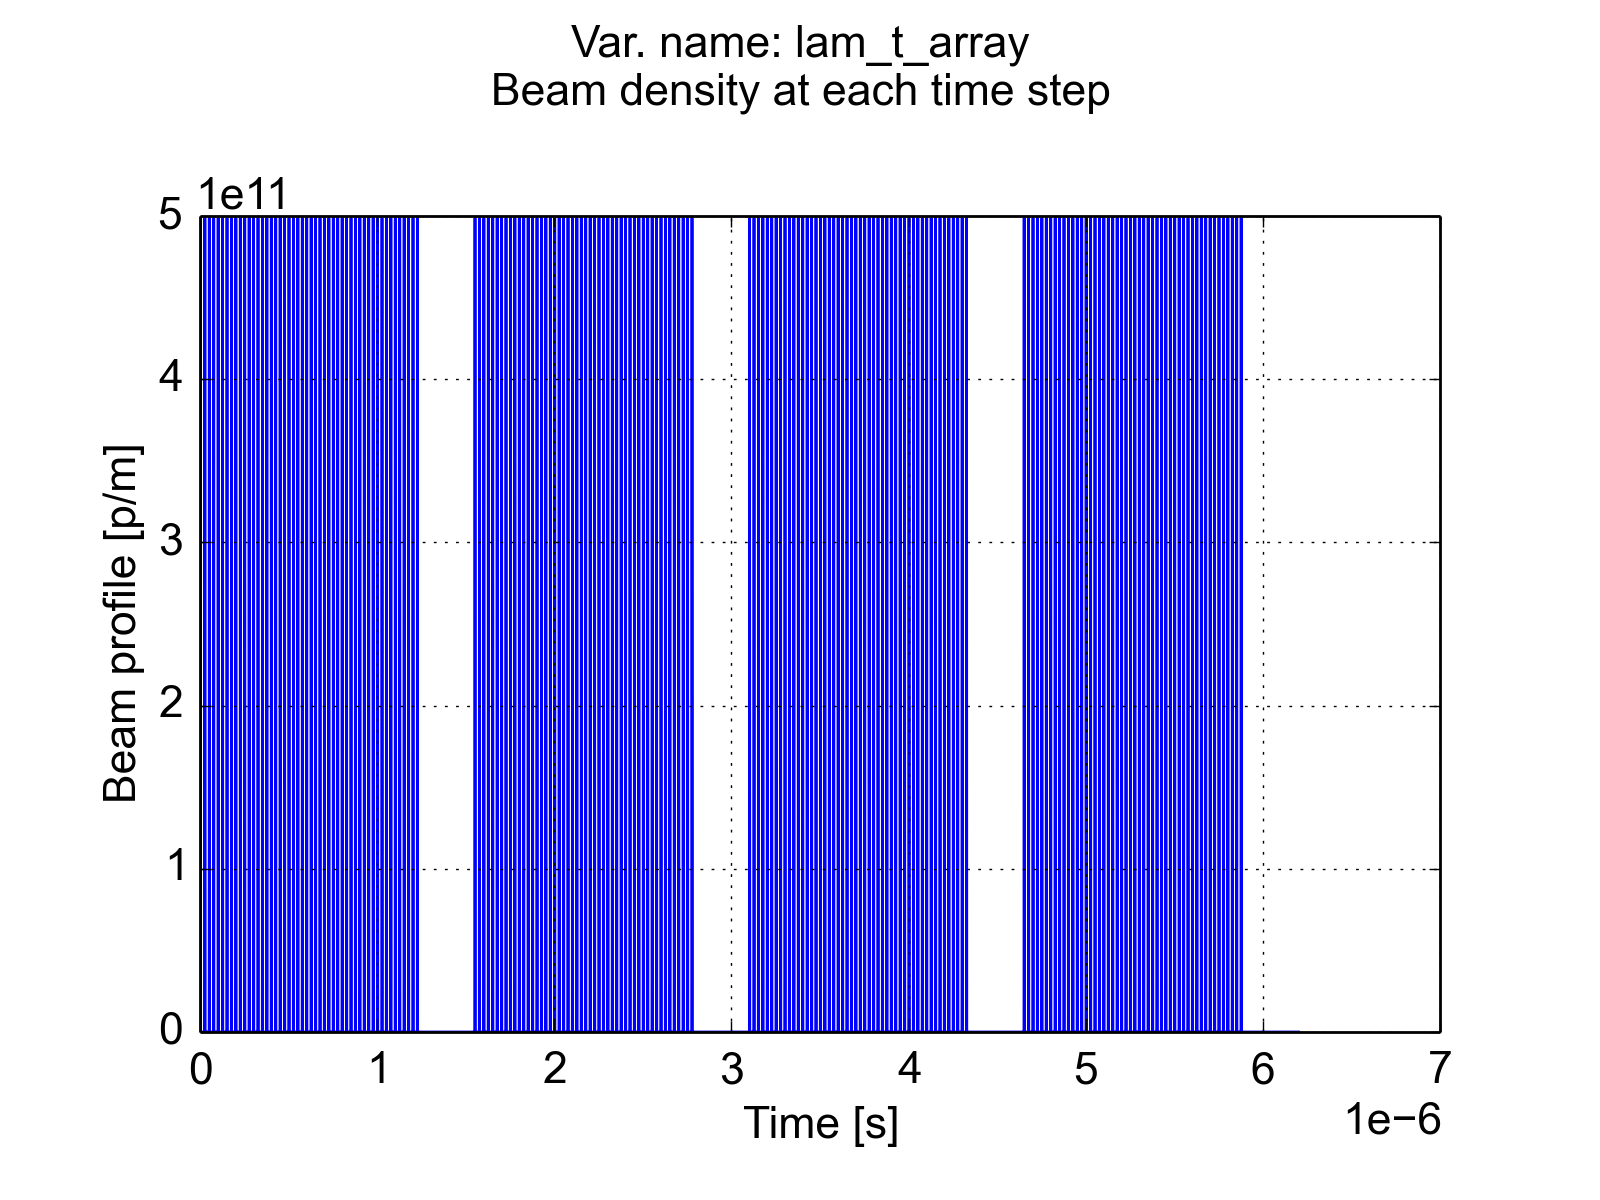
\includegraphics[trim = 0 0 0 0, clip, width=.95\textwidth]{../../example/fig01.png}
\end{center}
\end{figure}

\begin{figure}[p]
\begin{center}
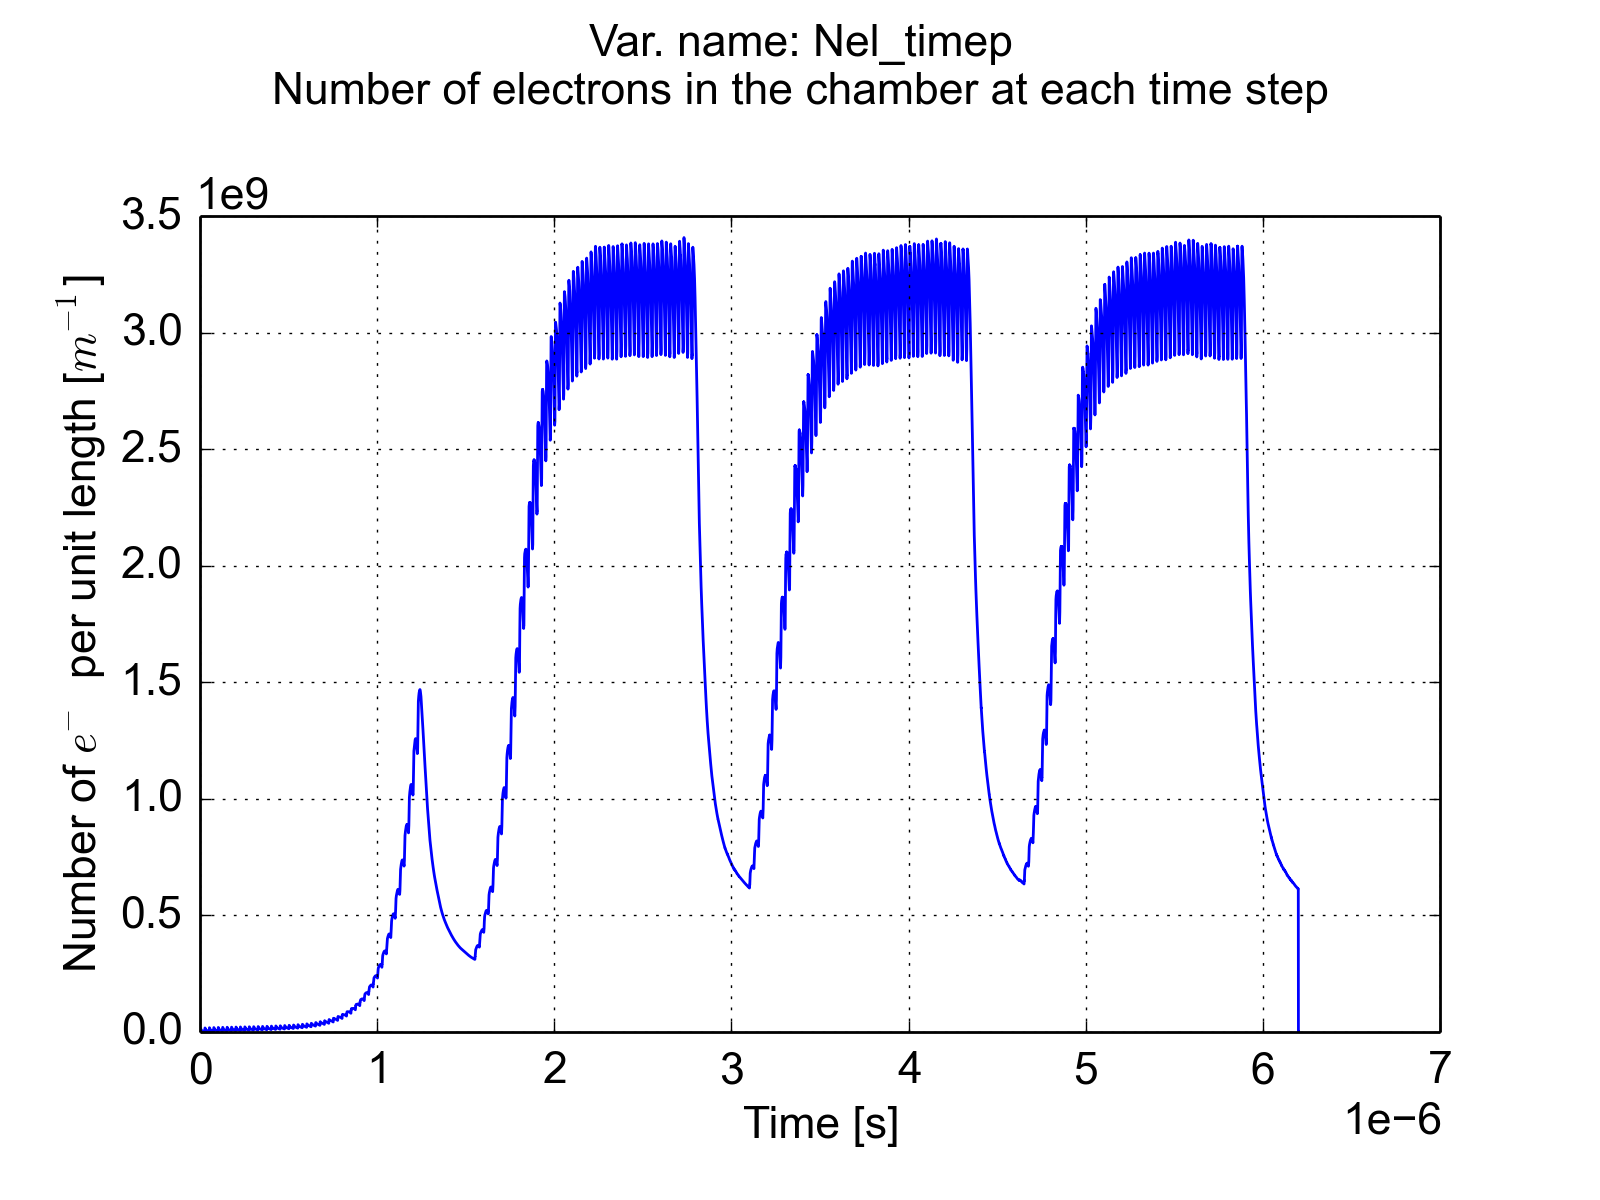
\includegraphics[trim = 0 0 0 0, clip, width=.95\textwidth]{../../example/fig02.png}
\end{center}
\end{figure}

\begin{figure}[p]
\begin{center}
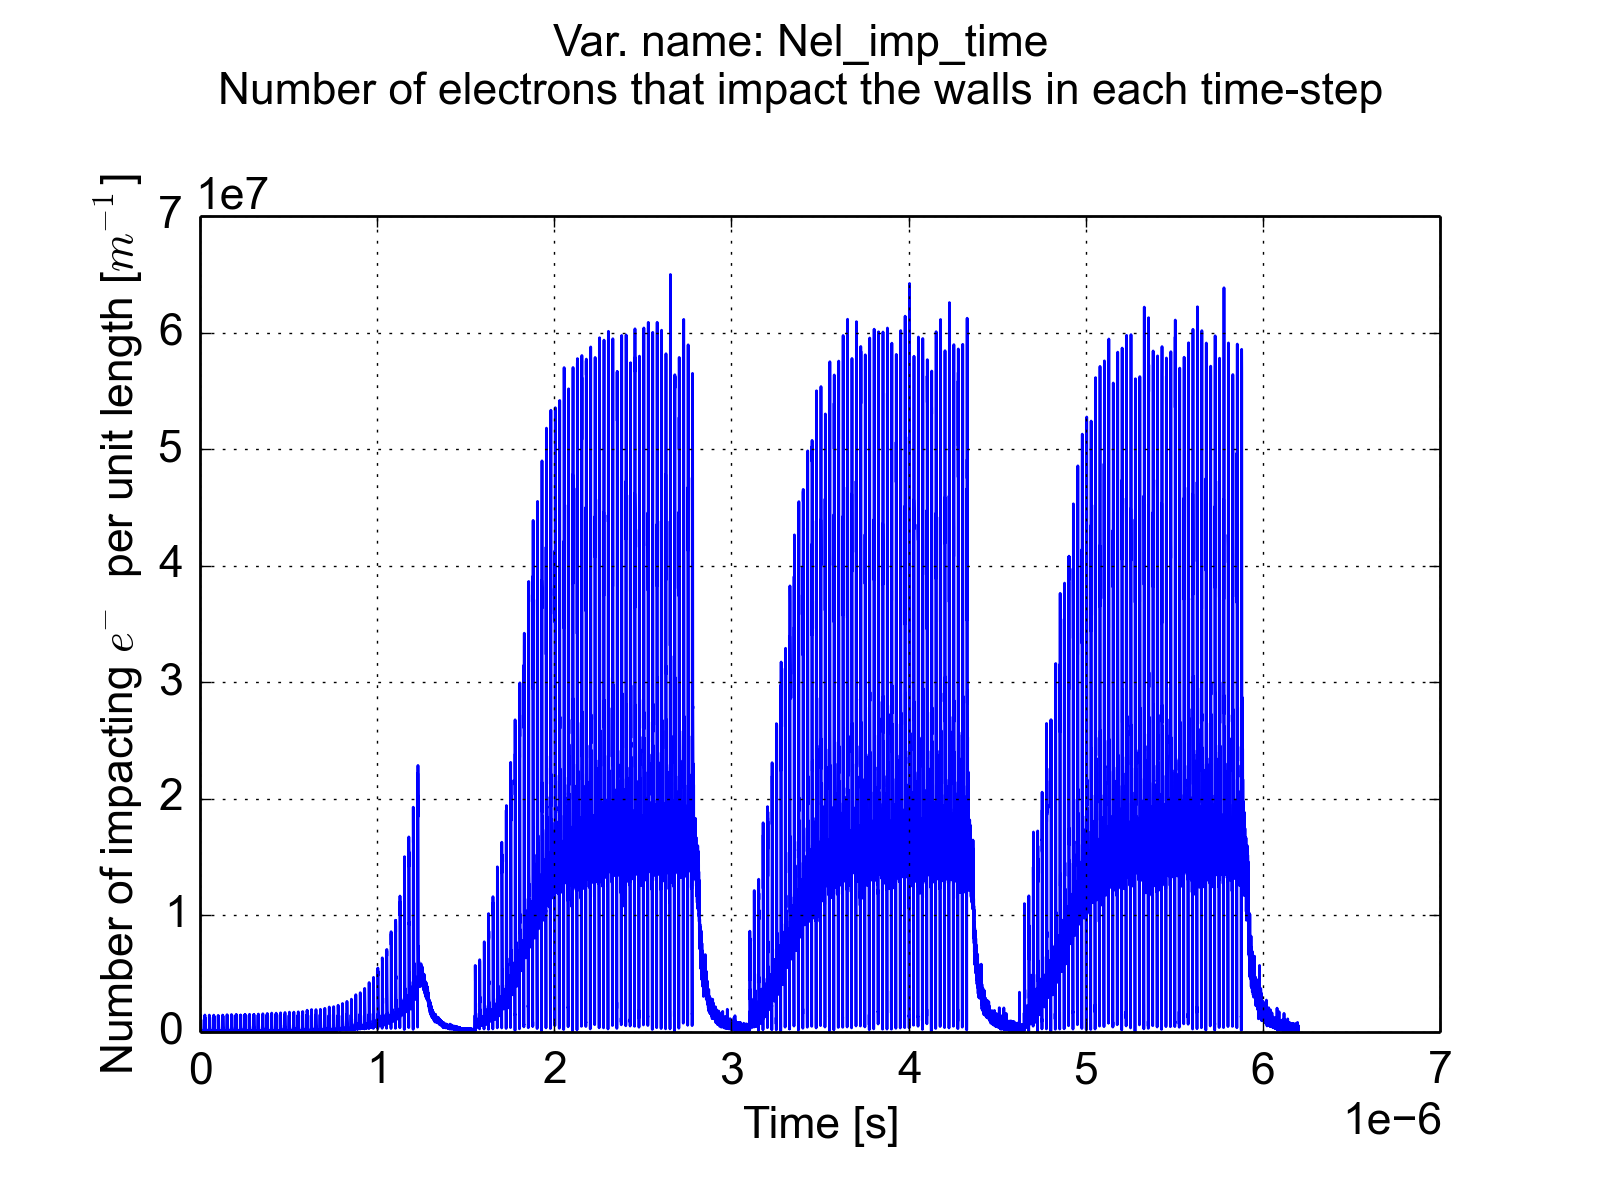
\includegraphics[trim = 0 0 0 0, clip, width=.95\textwidth]{../../example/fig03.png}
\end{center}
\end{figure}

\begin{figure}[p]
\begin{center}
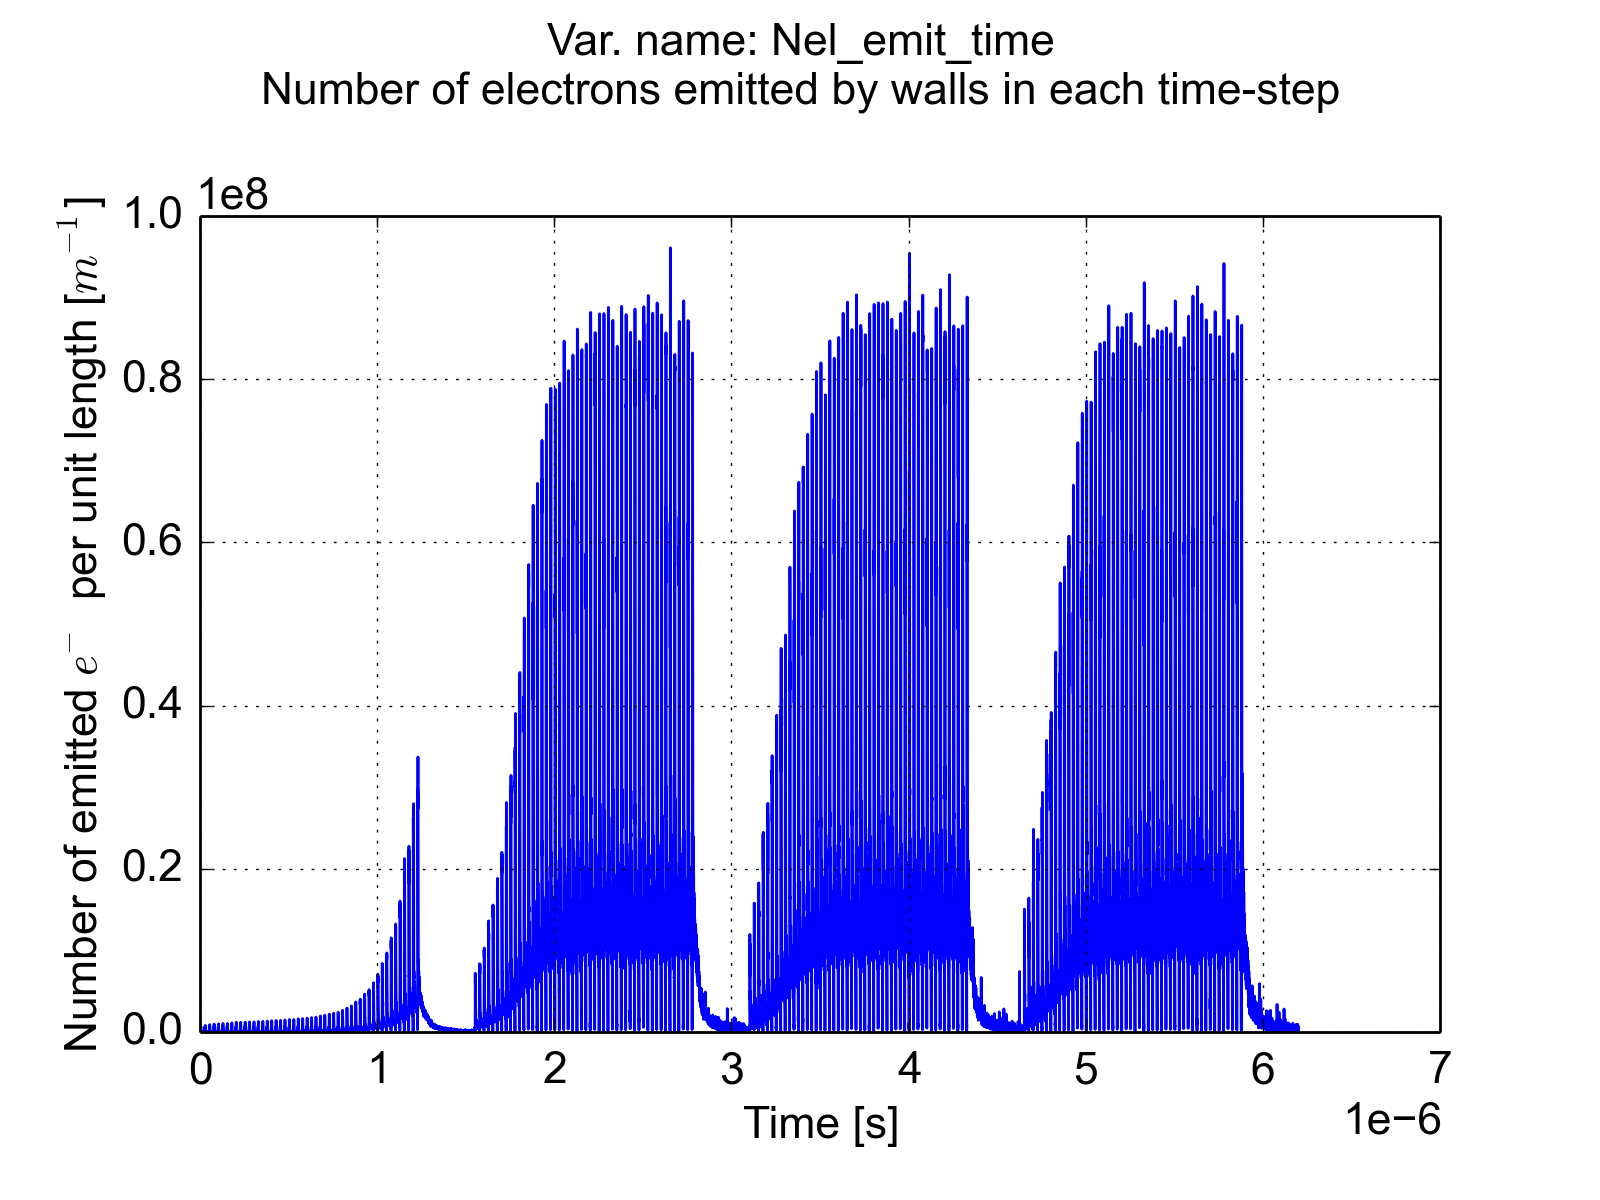
\includegraphics[trim = 0 0 0 0, clip, width=.95\textwidth]{../../example/fig04.png}
\end{center}
\end{figure}

\begin{figure}[p]
\begin{center}
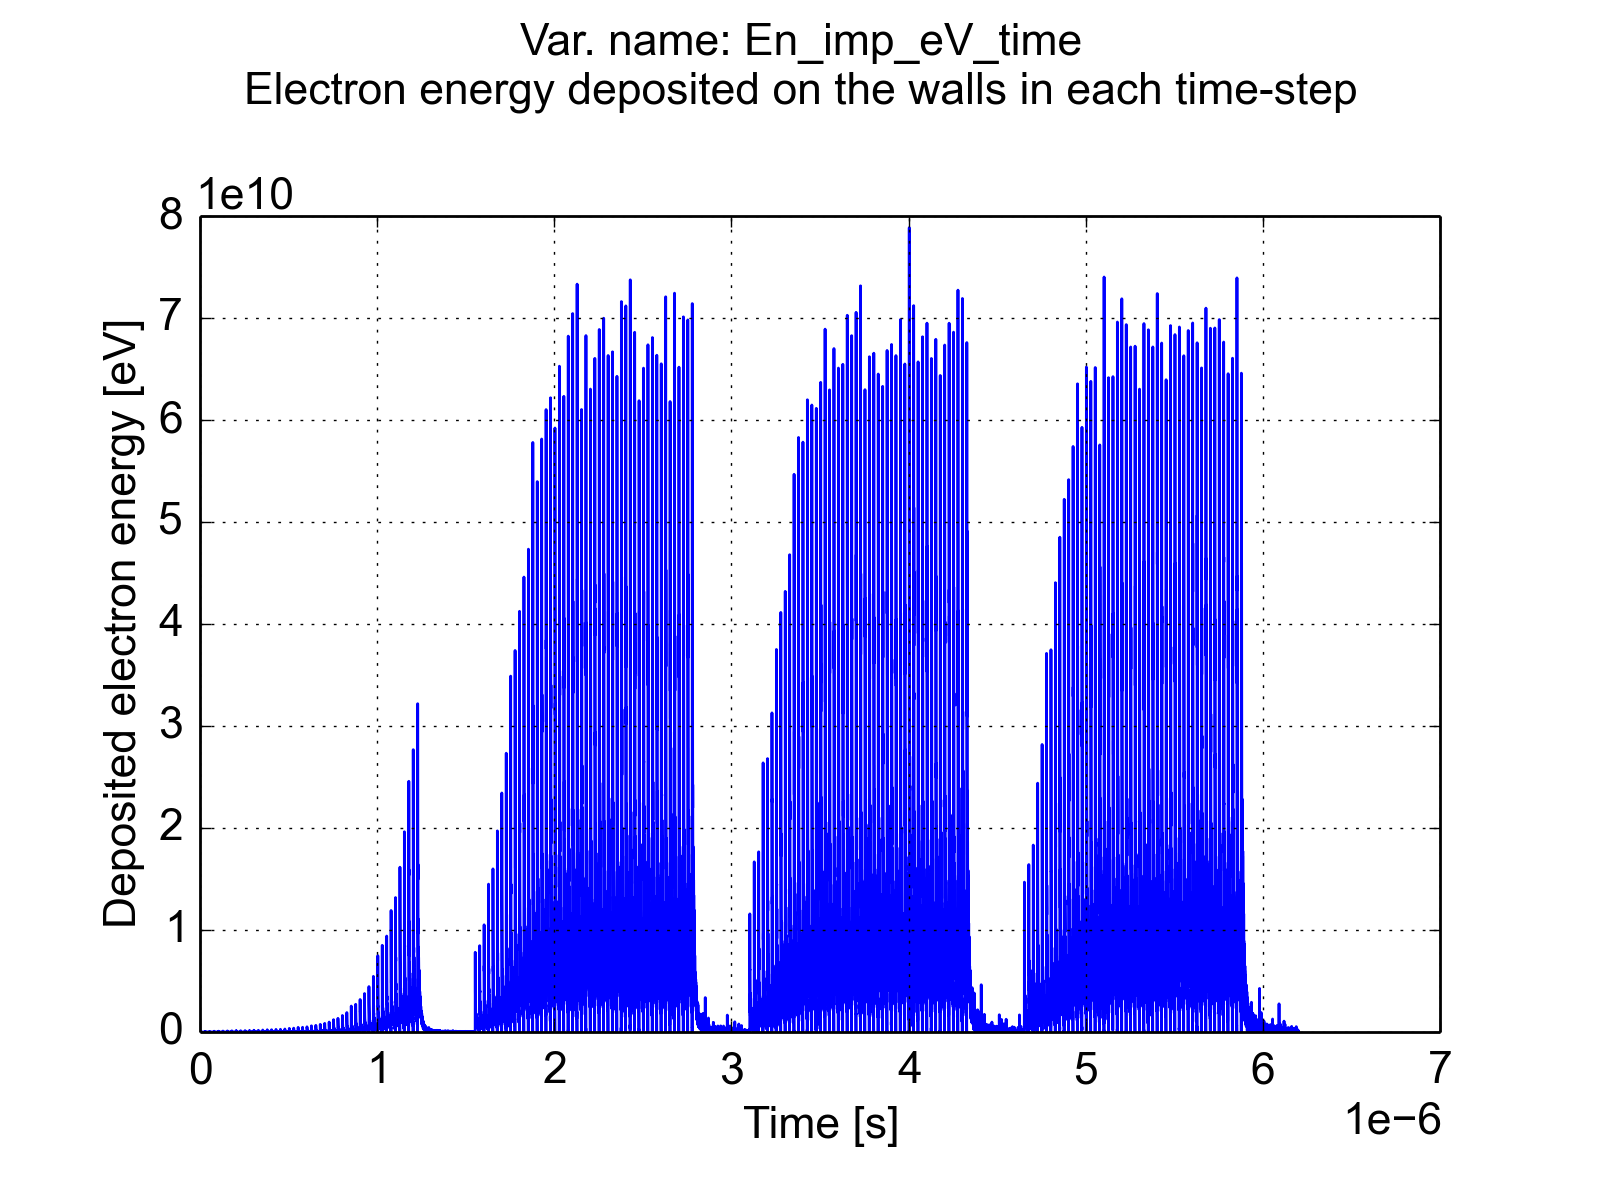
\includegraphics[trim = 0 0 0 0, clip, width=.95\textwidth]{../../example/fig05.png}
\end{center}
\end{figure}

\begin{figure}[p]
\begin{center}
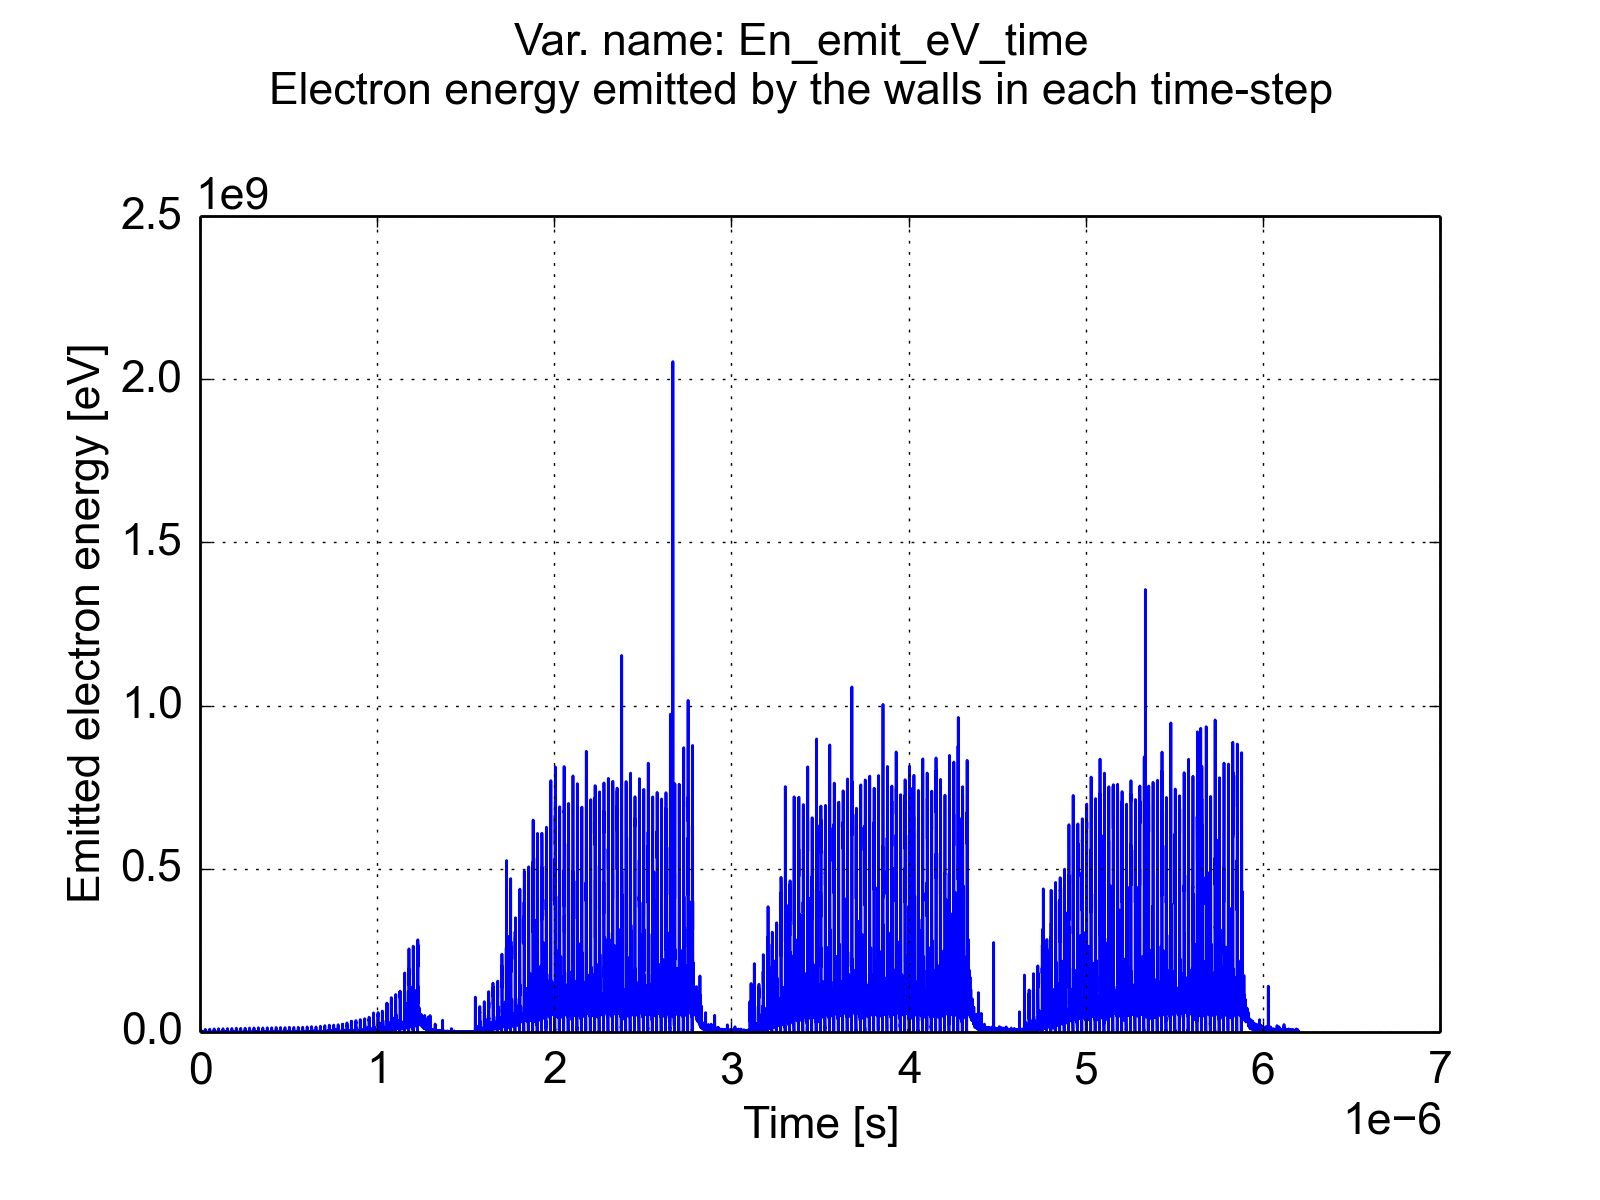
\includegraphics[trim = 0 0 0 0, clip, width=.95\textwidth]{../../example/fig06.png}
\end{center}
\end{figure}

\FloatBarrier

\begin{figure}[p]
\begin{center}
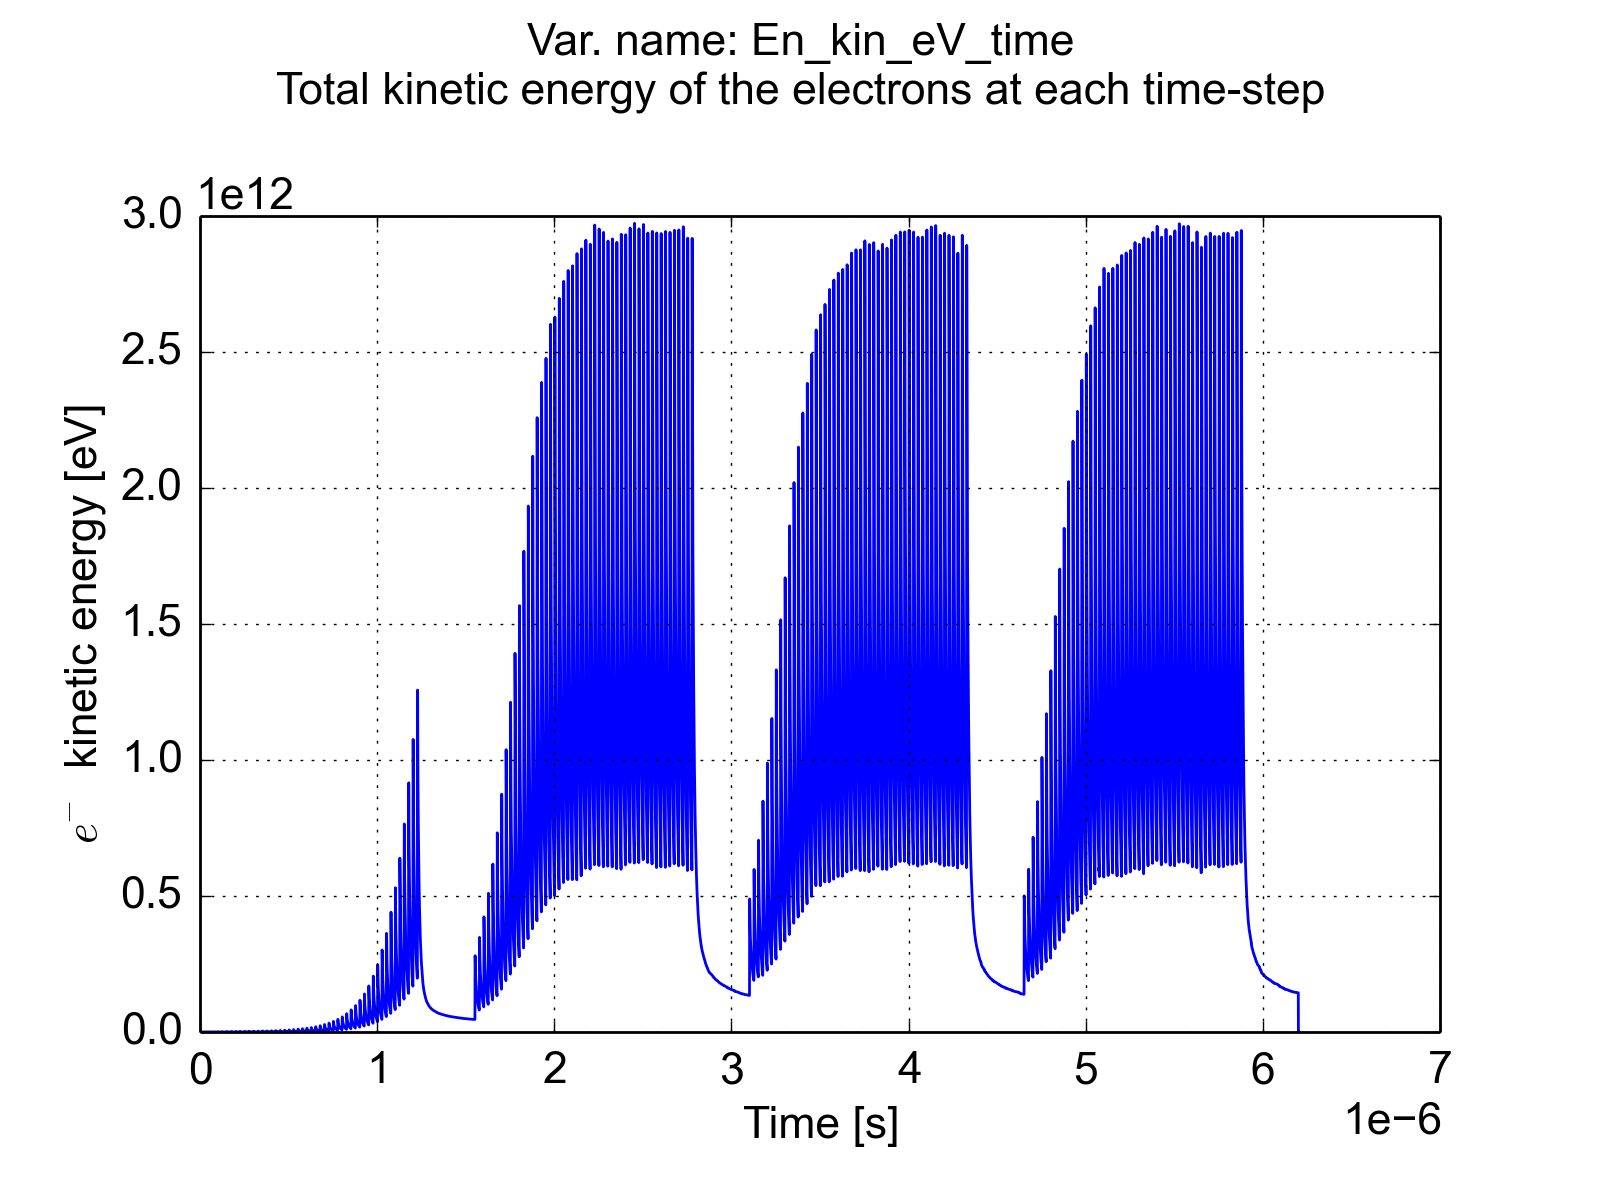
\includegraphics[trim = 0 0 0 0, clip, width=.95\textwidth]{../../example/fig07.png}
\end{center}
\end{figure}

\begin{figure}[p]
\begin{center}
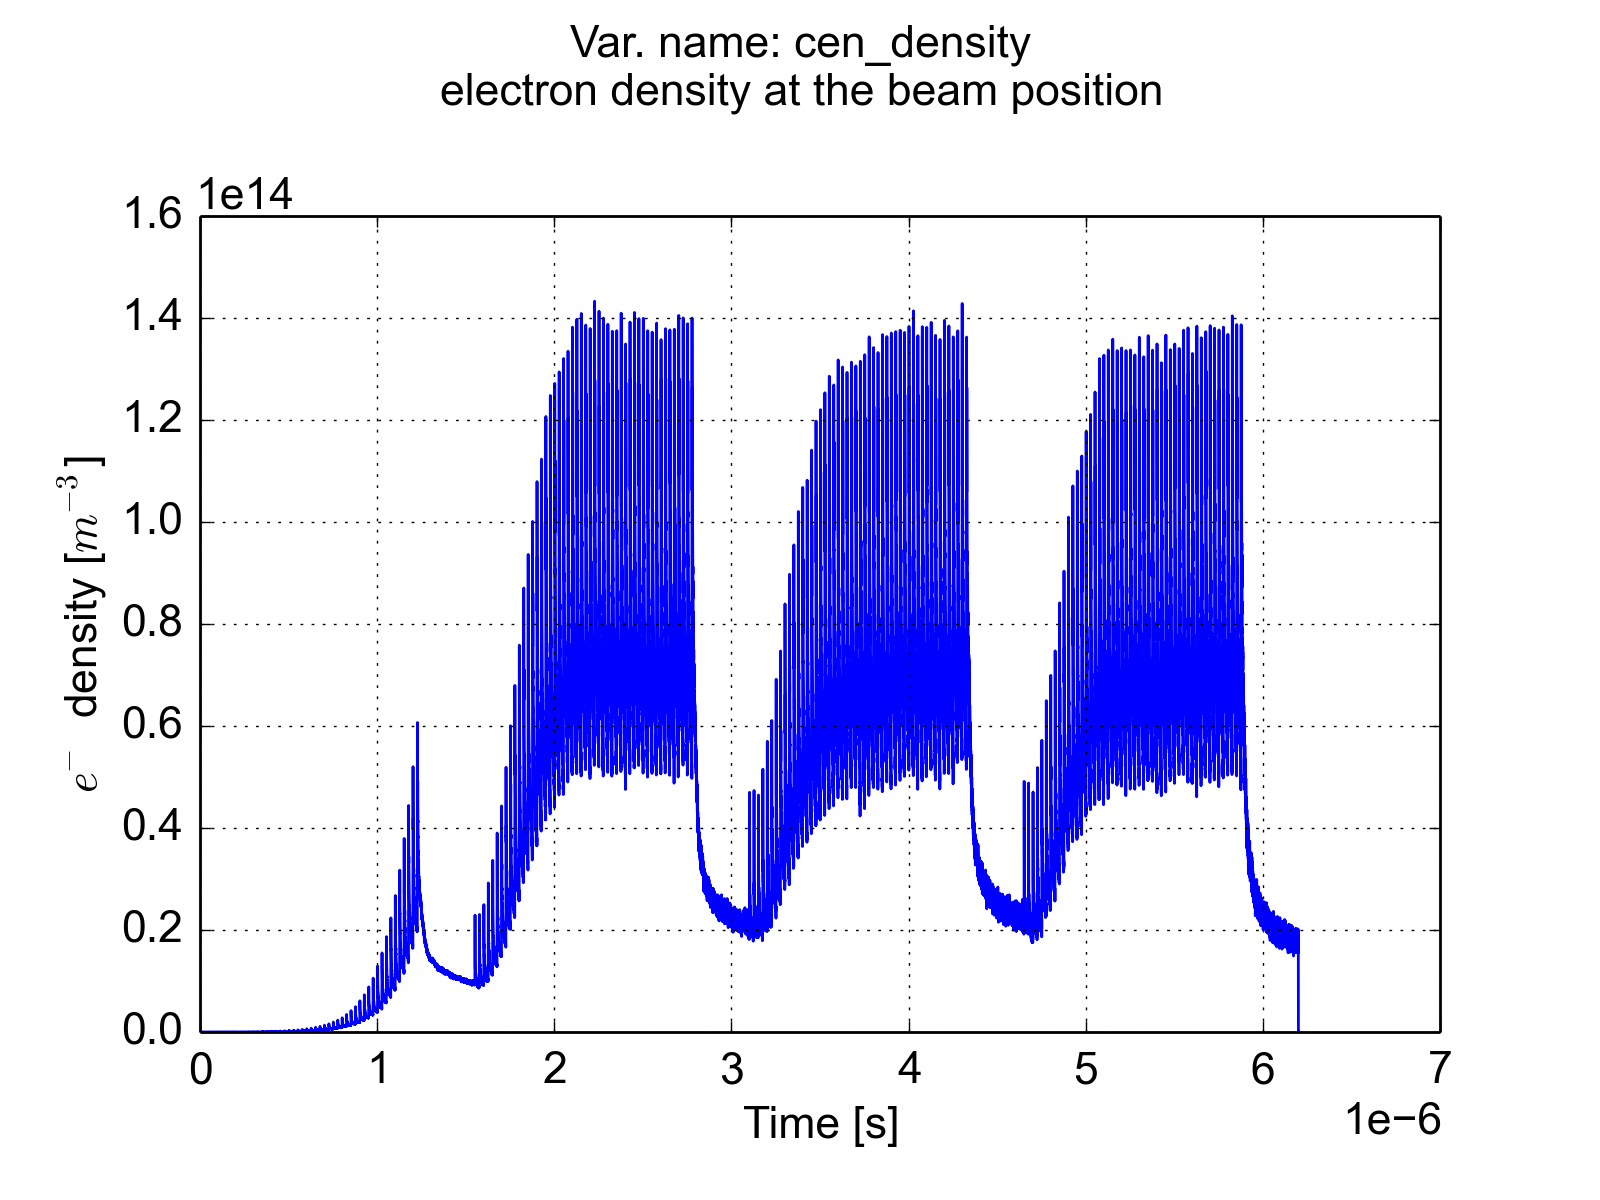
\includegraphics[trim = 0 0 0 0, clip, width=.95\textwidth]{../../example/fig08.png}
\end{center}
\end{figure}

\begin{figure}[p]
\begin{center}
\includegraphics[trim = 0 0 0 0, clip, width=.95\textwidth]{../../example/fig09.png}
\end{center}
\end{figure}

\begin{figure}[p]
\begin{center}
\includegraphics[trim = 0 0 0 0, clip, width=.95\textwidth]{../../example/fig10.png}
\end{center}
\end{figure}

\begin{figure}[p]
\begin{center}
\includegraphics[trim = 0 0 0 0, clip, width=.95\textwidth]{../../example/fig11.png}
\end{center}
\end{figure}

\begin{figure}[p]
\begin{center}
\includegraphics[trim = 0 0 0 0, clip, width=.95\textwidth]{../../example/fig12.png}
\end{center}
\end{figure}

\begin{figure}[p]
\begin{center}
\includegraphics[trim = 0 0 0 0, clip, width=.95\textwidth]{../../example/fig13.png}
\end{center}
\end{figure}

\begin{figure}[p]
\begin{center}
\includegraphics[trim = 0 0 0 0, clip, width=.95\textwidth]{../../example/fig14.png}
\end{center}
\end{figure}

\begin{figure}[p]
\begin{center}
\includegraphics[trim = 0 0 0 0, clip, width=.95\textwidth]{../../example/fig15.png}
\end{center}
\end{figure}

\begin{figure}[p]
\begin{center}
\includegraphics[trim = 0 0 0 0, clip, width=.95\textwidth]{../../example/fig16.png}
\end{center}
\end{figure}

\FloatBarrier

\begin{figure}[p]
\begin{center}
\includegraphics[trim = 0 0 0 0, clip, width=.95\textwidth]{../../example/fig17.png}
\end{center}
\end{figure}

\begin{figure}[p]
\begin{center}
\includegraphics[trim = 0 0 0 0, clip, width=.95\textwidth]{../../example/fig18.png}
\end{center}
\end{figure}

\FloatBarrier

\begin{figure}[p]
\begin{center}
\includegraphics[trim = 0 0 0 0, clip, width=.95\textwidth]{../../example/fig19.png}
\end{center}
\end{figure}

\begin{figure}[p]
\begin{center}
\includegraphics[trim = 0 0 0 0, clip, width=.95\textwidth]{../../example/fig20.png}
\end{center}
\end{figure}




\end{document}
\grid
